\chapter{Xarxes neuronals (artificials)}
\section{Introducció}
Models $y(x) = g(w^T \phi (x)),\ x \in \mathbb{R}^d, w \in \mathbb{R}^{d + 1}$.
$$
\phi(x) = 
\begin{pmatrix}
\phi_0(x) = 1 \\
\phi_1(x)\\
\vdots\\
\phi_M(x)
\end{pmatrix}
\quad 
g : f_n \ g:\mathbb{R} \rightarrow \mathbb{R} \text{(inversa global)}; 
\quad \phi : \mathbb{R}^d \rightarrow \mathbb{R}^M
$$
$$
X_{N \times d+ 1} \xrightarrow{\phi} \Phi_{N \times (M + 1)}
$$

La manera usual d'obtenir models \emph{no lineals} és establir funcions de base \emph{parametritzades}. La presència d'aquests paràmetres no lineals fa que les $\phi$ no es puguin pre-calcular.

En Xarxes Neuronals, la tria d'aquestes funcions de base es fa de la següent manera:
$$
\phi_i(x) := \phi (\psi(x, v_i))
$$
\begin{align*}
	&v_i & \text{és un vector de paràmetres (no lineals)} \\
	&\psi : \mathbb{R}^d \times \mathbb{R}^d \rightarrow \mathbb{R}
	& \text{és una funció de combinació} \\
	&\phi : \mathbb{R} \rightarrow (a,b) &
	\text{és una funció d'activació}
\end{align*}

$\psi$ calcula una similitud entre dos vectors: $x_1 v_i$.
$\phi$ determina el valor final d'activació de $\phi_i$.

\textbf{Definició}: diem que una funció $\phi \mathbb{R} \rightarrow (a,b)$ és \emph{sigmoidal} si:
\begin{enumerate}
	\item $\lim\limits_{z \rightarrow - \infty} \phi(b) = a$
	\item $\lim\limits_{z \rightarrow + \infty} \phi(z) = b$
	\item $\phi'(z) > 0,\ \forall z \qquad \phi'(z) < 0,\ \forall z$ i $\phi'$ té forma de campana.
\end{enumerate}

\textbf{Exemples}:

\begin{enumerate}
	\item La funció logística $\phi(z) = \frac{1}{1 + e^{-z}} \in (0, 1)$
	\begin{figure}[H]
		\centering
		\begin{tikzpicture}
		\begin{axis}[
		xmin=-7,xmax=7,ymin=0,ymax=1,
		domain=-10:10,
		axis x line=center,
		axis y line=center
		]
		\addplot+[mark=none] {1/(1 + exp(-x))};
		\end{axis}
		\end{tikzpicture}
		\caption{Gràfic funció logística}
		\label{fig:logistic}
	\end{figure}

	\item La tangent hiperbòlica $\phi(z) = \frac{e^z - e^{-z}}{e^z + e^{-z}} \in (0,1)$.
	
	\begin{figure}[H]
		\centering
		\begin{tikzpicture}
		\begin{axis}[
		xmin=-5,xmax=5,ymin=-1.05,ymax=1.05,
		domain=-5:5,
		axis x line=center,
		axis y line=center
		]
		\addplot+[mark=none] {(exp(x) - exp(-x))/(exp(x) + exp(-x))};
		\end{axis}
		\end{tikzpicture}
		\caption{Gràfic funció inversa hiperbòlica}
		\label{fig:inv_hiperbol}
	\end{figure}
\end{enumerate}

$$
\implies y(x) = g(w^T \phi(x)) = g\left(\sum_{i=0}^M w_i \phi_i(x)\right) = g \left( \sum_{i=0}^M w_i \phi(v_i^T x + v_{i0}) \right)
$$
\begin{itemize}
	\item $w_i$ són paràmetres lineals
	\item $v_i$ i $v_{i0}$ són paràmetres no lineals
\end{itemize}

% FIGURA 1

Si es dediquen esforços a optimitzar una funció que té molts mínims locals es pot arribar a un mínim que no sigui un mínim absolut. Això dificulta molt la feina d'optimització. Tot i així l'error al que s'acaba arribant al final resulta ser només un error amb les dades d'entrenament. 

Per tant, amb les dades més genèriques l'error també serà menor. Si es minimitzessin al màxim les dades d'entrenament llavors amb les altres potser no s'aconsegueix un mínim.

% FIGURA 2

A cada $ \phi_i(x) $ se li diu \emph{neurona}.

\begin{figure}[H]
	\centering
	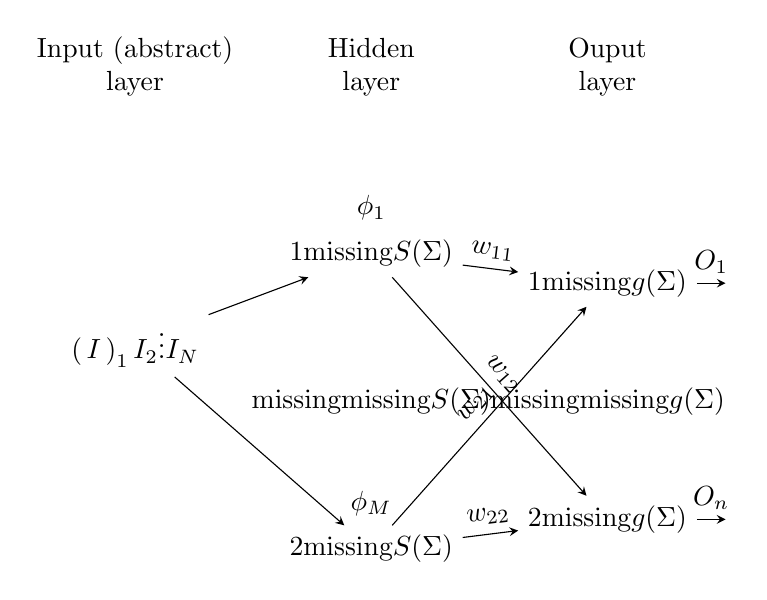
\begin{tikzpicture}[x=1.5cm, y=1.5cm, >=stealth]
	
	
	\node (input) at (0,0) {$
		\begin{pmatrix}
		I_1 \\ I_2 \\ \vdots \\ I_N
		\end{pmatrix}
		$};
		
	\foreach \m [count=\y] in {1,missing,2}
	\node [every neuron/.try, neuron \m/.try ] (hidden-\m) at (2,2-\y*1.25) {\ifthenelse{\equal{\m}{missing}}{}{$S(\Sigma)$}};
	
	\foreach \m [count=\y] in {1,missing,2}
	\node [every neuron/.try, neuron \m/.try ] (output-\m) at (4,1.5-\y) {\ifthenelse{\equal{\m}{missing}}{}{$g(\Sigma)$}};
	
	\foreach \l [count=\i] in {1,M}
	\node [above] at (hidden-\i.north) {$\phi_\l$};
	
	\foreach \l [count=\i] in {1,n}
	\draw [->] (output-\i) -- ++(1,0)
	node [above, midway] {$O_\l$};
	
	\foreach \i in {1,...,2}
	\draw [->] (input) -- (hidden-\i);
	
	\foreach \i in {1,...,2}
	\foreach \j in {1,...,2}
	\draw [->] (hidden-\i) -- (output-\j) node [midway,above,sloped] {$w_{\i\j}$};
	
	\foreach \l [count=\x from 0] in {Input (abstract), Hidden, Ouput}
	\node [align=center, above] at (\x*2,2) {\l \\ layer};
	
	\end{tikzpicture}
\end{figure}

\begin{itemize}
	\item La xarxa treballa "endavant" quan ho fa en el sentit de les fletxes $\rightarrow$.
	\item La capa de \emph{sortida} és la darrera capa endavant
	\item Les capes \emph{ocultes} són totes excepte la de sortida (les seves \emph{neurones} també es diuen \emph{ocultes}).
	\item No hi ha capa "d'entrada".
\end{itemize}

A vegades tenim múltiples capes ocultes

\begin{figure}[H]
	\centering
	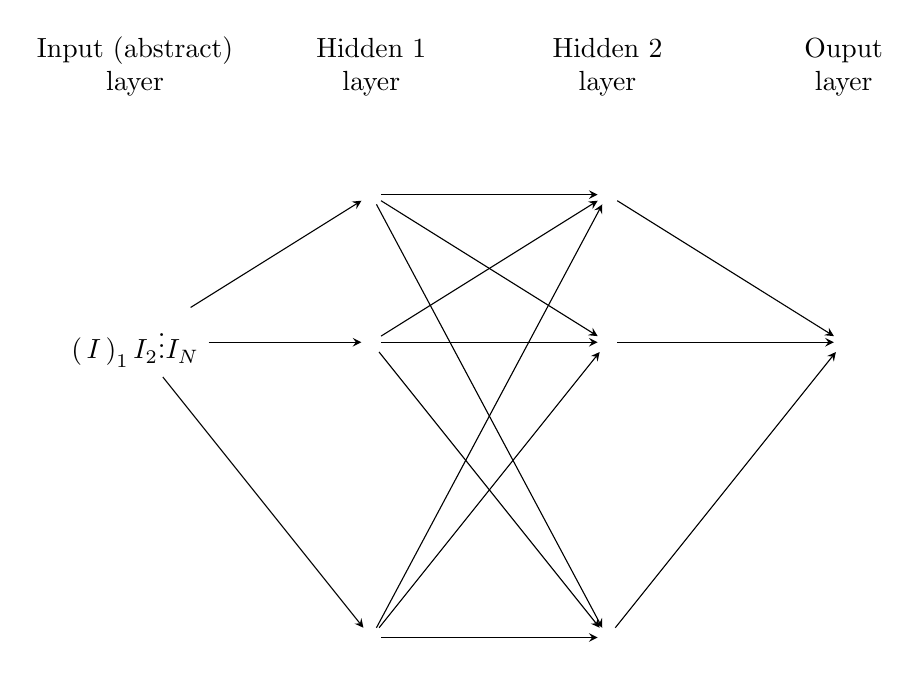
\begin{tikzpicture}[x=1.5cm, y=1.5cm, >=stealth]
		\node (input) at (0,0) {$
			\begin{pmatrix}
			I_1 \\ I_2 \\ \vdots \\ I_N
			\end{pmatrix}$};
		
		\foreach \m [count=\y] in {1,2,missing,3} 
		\node [every neuron/.try, neuron \m/.try](hidden-1-\m) at (2,2.5 - \y*1.25){};
		
		\foreach \m [count=\y] in {1,2,missing,3} 
		\node [every neuron/.try, neuron \m/.try](hidden-2-\m) at (4,2.5 - \y*1.25){};
		
		\node [every neuron/.try](output) at(6,0){};
		
		\foreach \i in {1,...,3}
		{
			\draw[->](input) -- (hidden-1-\i); 
			\draw[->](hidden-2-\i) -- (output); 
			\foreach \j in {1,...,3}
			{ 	
				\draw[->](hidden-1-\i) -- (hidden-2-\j);
			}
		}
	
		\foreach \l [count=\x from 0] in {Input (abstract), Hidden 1, Hidden 2, Ouput}
		\node [align=center, above] at (\x*2,2) {\l \\ layer};
	\end{tikzpicture}
\end{figure}

$$
y(x) = g\left(\sum_i w_i\phi_i(x)\right) =
g\left(\sum_i w_i \phi (v_i^T x) \right) =
g\left( \sum_i w_i \phi \left(\sum_j v_{ij} x_j\right)  \right)
$$
En aquest cas $x_j \rightarrow \gamma_i (x) = \phi (z_j^T x + z_{j0})$. Per tant:
$$
y(x) = g\left( \sum_i w_i \phi \left( \sum_j w_{ij} \phi \left( z_{jn} x_n + x_{n0} \right) + v_{j0} \right) + w_0 \right)
$$

\subsection{La funció g}

\begin{table}[H]
	\centering
	\setlength\extrarowheight{15pt}
	\begin{tabular}{p{2.2cm}|p{2.3cm}p{3cm}p{2.8cm}}
		& Regressió & \parbox{2cm}{Classificació \\ ($K=2$)} & \parbox{2cm}{Classificació \\ ($K > 2$)} \\
		\hline
		Funció g & g = Identitat & logística & softmax \\
		Funció d'error & error quadràtic & entropia creuada & entropia creuada generalitzada \\
		Interpretació de la sortida & el target K-èsim (m neurones de sortida) & \parbox{3cm}{$y(x) = P(w_1 |X)$ \\ $\implies$ \\ $P(w_2|X) = 1 - g(x)$} (una neurona de sortida) &  \parbox{2.8cm}{$y_k(x) = P(w_k|X)$ \\ (K neurones de sortida)}
	\end{tabular}
\end{table}

\section{Entrenament de xarxes neuronals (Xarxes MLD)}
$$
y_{MLD}(x) = 
\begin{pmatrix}
y_1(x) \\
y_2(x) \\
\vdots \\
y_m(x)
\end{pmatrix},
\  x \in \mathbb{R}^d 
\quad y_{MLD}: \mathbb{R}^d \rightarrow \mathbb{R}^m
$$

\begin{itemize}
	\item Es tenen $c$ capes ocultes i 1 capa de sortida = $c + 1$ capes.
	\item $w_l$ és el nombre de neurones de la capa $l$
\end{itemize}

\begin{figure}[H]
	\centering
	\begin{tikzpicture}[x=1.5cm, y=1.5cm]
		\node[every neuron/.try] (i) at (0,0) {i};
		\node[every neuron/.try] (j) at (2,0) {j};
		\node[below = 0.3cm of i] {$(l - 1)$};
		\node[below = 0.3cm of j] {$(l)$};
		\draw[->] (i) to[bend left = 20] node[midway,above] {$w_{ji}^l$} (j);
	\end{tikzpicture}
\end{figure}
\begin{itemize}
	\item $\boldsymbol{w_l} = \begin{pmatrix}
	w_{ji}^l
	\end{pmatrix}_{j,i} \rightarrow$ vector $\forall$ parella $j,i$.
	\item $W = (w_l)_{l=1,...,c}$.
\end{itemize}


Es defineix:
\begin{align*}
	& z_j^l := \phi(a_j^l) \\
	& a_j^l := \sum_{i=0}^{h_{l-1}} w_{ji}^l z_i^{l-1}
\end{align*}

Es fixa l'exemple $n$. El primer que es fa és calcular les sortides de totes les neurones de la xarxa. Primer es calculen totes les $\delta_k$ de totes les $c$ capes ocultes.

\begin{align*}
	& \delta_k^{c+1} = t_{nk} - z_{k}^{c+1} \\
	& \delta_j^{l+1} \propto \sum_{k} w_{kj}^{l+1} · \delta_{k}^{c+1} \\
	& \Delta w_{kj}^{l+1} \propto \delta_k^{c+1} z_j^{l+1}	
\end{align*}

\begin{figure}[H]
	\centering
	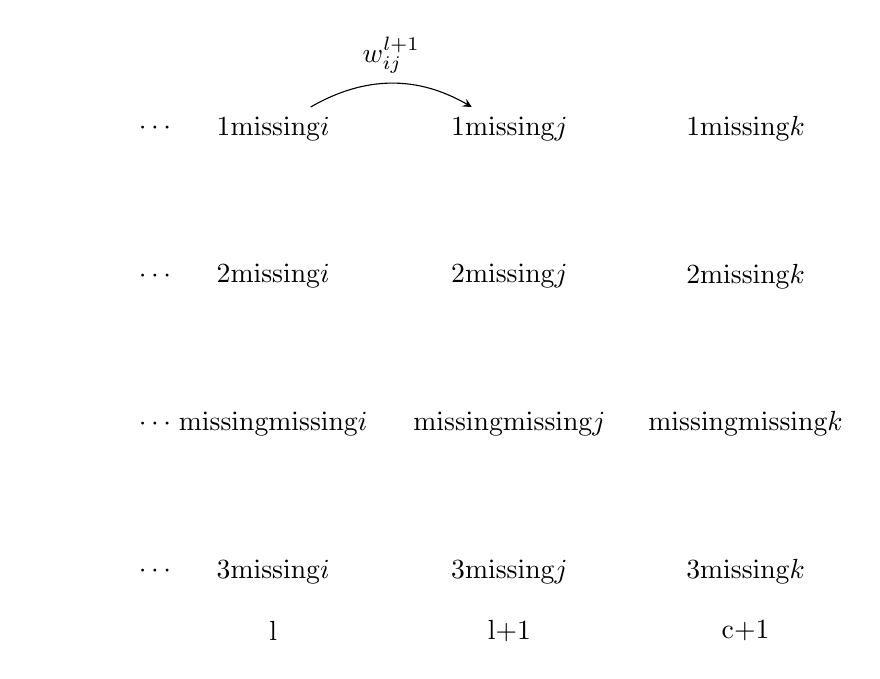
\begin{tikzpicture}[x=1.5cm, y=1.5cm, >=stealth]
		\foreach \m [count=\y] in {1,2,missing,3}
		\node[every neuron/.try, neuron \m/.try](hidden-0-\m) at (0,2.5 - \y*1.25){};
		
		\foreach \m in {1,...,4}
		\node(intermid-\m) at (1,2.5 - \m*1.25){$\cdots$};
		
		\foreach \m [count=\y] in {1,2,missing,3}
		\node[every neuron/.try, neuron \m/.try](hidden-1-\m) at (2,2.5 - \y*1.25)
		{\ifthenelse{\equal{\m}{missing}}{}{$i$}};
		
		\foreach \m [count=\y] in {1,2,missing,3}
		\node[every neuron/.try, neuron \m/.try](hidden-2-\m) at (4,2.5 - \y*1.25)
		{\ifthenelse{\equal{\m}{missing}}{}{$j$}};
		
		\foreach \m [count=\y] in {1,2,missing,3}
		\node[every neuron/.try, neuron \m/.try](hidden-3-\m) at (6,2.5 - \y*1.25)
		{\ifthenelse{\equal{\m}{missing}}{}{$k$}};
		
		\foreach \m [count=\y] in {l, l+1, c+1}
		\node at (2*\y, -3){\m};
		
		\draw[->](hidden-1-1) to[out=30, in=150] node [sloped,midway,above]{$w_{ij}^{l+1}$} (hidden-2-1) ;
	\end{tikzpicture}
\end{figure}

\subsection{Algorisme \texttt{backprop}}

\texttt{backprop(D, "especificació de l'arquitectura")}

\begin{algorithmic}
	\State inicialitzar els pesos  $\forall j,l,i$
	\Repeat
	\For{$n := 1$ fins $N$} 
		\Comment{PAS FORWARD (sentit de les fletxes)}
		\State Calcular les sortides $z_j^l,\ \forall j,l$
		\Comment{PAS BACKWARD}
		\For{$l := c$ fins $1$}
			\If{$l = c$} 
				$\delta_j := (t_{nj} - z_{j}^{c+1})$
			\Else
				$\ \delta_j^l := \phi' (a_j^l) \sum_q w_{qj}^{l+1} z_j^l$
			\EndIf
		\EndFor
	\EndFor
	\ForAll{j,l,i}
		\State $\Delta w_{ji}^l := \sum_{n=1}^N \Delta w_{ji}^l$
		\State $w_{ji}^l := w_{ji}^l - \alpha \Delta w_{ji}^l$
	\EndFor
	\Until{Convergeixi}
\end{algorithmic}

\section{Xarxes de neurones de Base Radial}
RBF (\textsc{Radial Basis Function})

\begin{align*}
& \phi_i (x) = \phi\left( \frac{||x - m_i||}{h_i} \right)
\begin{cases}
h_i > 0: &\text{ paràmetre de suavització} \\
m_i: &\text{centre de la neurona } i
\end{cases} \\
& \phi:\mathbb{R}_0^+ \rightarrow \mathbb{R} \\
& \phi(z) = \exp\left( - \frac{z^2}{2} \right)
\end{align*}

\begin{figure}[H]
	\centering
	\begin{tikzpicture}
		\begin{axis}[
		xmin=-0,xmax=5,ymin=0,ymax=1.05,
		domain=0:5,
		samples=100,
		axis x line=center,
		axis y line=center
		]
		\addplot+[mark=none] {exp(-x^2/2))};			
		\end{axis}
	\end{tikzpicture}
\end{figure}
\subsection{Entrenament d'una xarxa RBF}
\subsubsection{Posicionar les neurones a l'espai d'entrada}
Usant un algorisme de \emph{clustering} (per exemple \texttt{k-means}), amb un nombre de clusters (M). Uaser el resultat del clustering per determinar:
\begin{itemize}
	\item Centre des les M neurones: centroides del clustering ($m_i$)
	\item Paràmetres de suavització ($h_i$).
	\begin{align*}
		& h_i \propto \frac{d_{\max}}{\sqrt{2M}} \qquad d_{\max}\ \text{entre centres (ct.)} \\
		& h_i \propto d_{mitjana} \ \text{entre centres (ct.)} \\
		& h_i \propto d_{mitjana} \ \text{entre el $m_i$ i les dades $x_n$ (diferent per cada i)}
	\end{align*}
\end{itemize}

\subsubsection{Tenim les funcions $\phi_i (x) = \phi\left( \frac{||x - m_i||}{h_i} \right)$}
\begin{itemize}
	\item Calculem la matriu de disseny $\Phi_{ij} = \phi_j(x_i)$.
\end{itemize}
\subsubsection{Regressió en $\Phi$}
\begin{itemize}
	\item regressió: regressió lineal regularitzada (ridge regression)
	\item classificació ($k=$ 2 classes): regressió logística
	\item classificació ($k>$ 2 classes): regressió multilineal
\end{itemize}

$$
y_{RBF}(x) = \sum_{i=1}^{M} w_i \phi_i(x) + w_0 \quad \text{(regressió lineal)}
$$

\subsection{Influència de $M$ i $\{h_i\}$}
\begin{itemize}
	\item $M$ neurones $\rightarrow$ sobreajust (a menys que hi hagi regularització)
	\item $h_i$?
\end{itemize}

$$
\phi_i(x) = \exp\left( - \frac{||x - m_i||^2}{h_i^2} \right)
$$

% FIGURA 1
Imaginem que tenim una funció i una sèrie de dades i es fa un clustering d'aquestes dades. Es posen unes quantes neurones i cadascuna d'aquestes té una resposta Gaussiana. 

El paràmetre de suavització fa que les Gaussianes siguin més estretes o més amples. Si es tria una $h_i = h$ per totes les neurones i llavors es fa que $h \rightarrow \infty$ llavors la resposta de totes les neurones serà molt plana i la resposta de la xarxa serà l'infra-ajust.

Per contra si la $h \rightarrow 0$ la resposta de les neurones serà molt local i la xarxa tendirà al sobre-ajust.
